\chapter{Planning integration} % add folder structure
\label{cha:planningbridge}

This chapter aims to \textbf{integrate} the planning part developed by \textit{Filippo Rossi}\footnote{His entire project is described in \autoref{sub:planning}}\cite{fr}. What has already been discussed in the previous chapters leads to a \textbf{working} version of the robot (it is able to move around), but has no practical use, because you need to set \textbf{where} you want the robot to go \textbf{every time}. This is the goal of this chapter: add some \textbf{mission controls}, to give the robot some tasks it has to complete, without the need for any \textbf{low-level human interaction}.

\section{Modifications from original planning}

When the planning was developed, Filippo could not receive any feedback, since we were facing other challenges (i.e. make robots move independently). So, in response, the planning is more like a \textbf{generic workspace} to which we can add some \textbf{modifications} to meet our specific needs; then we can attach the \textbf{adapted workspace} to what has been already developed.

% aggiungere entrance tag per entrata porta, dato che non è ben definita

\subsection{Change JSON structure}
\label{sub:json}

Thanks to Filippo's \textbf{waypoints extractor} and \code{cvat} \textbf{annotation software}, all the coordinate information can be found in a \textbf{JSON file}: when the robot is told to move to a certain room, the only step to take is \textbf{looking} for its name in the file and read the \textbf{coordinates}.

But, because this JSON file was written as a \textbf{list of dictionaries}, you would need to iterate \textbf{on each element} and search for the one with the \textbf{desired name}, and when they match, you can the coordinates. Instead, for easier use, a dictionary was created with the name of the room as a \textbf{key} and the coordinates of its center and its boundaries as a \textbf{value}. Also, the coordinates on the Z axis have been removed because they are the same for all rooms. A comparison is shown in \autoref{lst:origjson} and \autoref{lst:modjson}. This was done with the \code{Python} script shown in \autoref{lst:script}.

\noindent\begin{minipage}{0.425\textwidth}
\noindent\begin{lstlisting}[
    language=json,
    style=jsonStile,
    caption={Original JSON structure},
    label={lst:origjson}]
[
    {
        "label": "povo_1_258",
        "center": [
            -11.749180327868853,
            -35.01639344262295,
            1.5
        ],
        "max": [
            -8.0,
            -30.5,
            1.5
        ],
        "min": [
            -15.5,
            -40.0,
            1.5
        ]
    },
    ...
]
\end{lstlisting}
\end{minipage}
\noindent\begin{minipage}{0.15\textwidth}
    \centering
    \noindent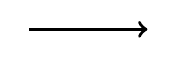
\begin{tikzpicture}
        \draw[->, very thick] (0,0) -- (1.5,0);
    \end{tikzpicture}
\end{minipage}
\noindent\begin{minipage}{0.425\textwidth}
\noindent\begin{lstlisting}[
    language=json,
    style=jsonStile,
    caption={Modified JSON structure},
    label={lst:modjson}]

{
    "povo_1_258": {
        "center": [
            -11.749180327868853,
            -35.01639344262295

        ],
        "max": [
            -8.0,
            -30.5

        ],
        "min": [
            -15.5,
            -40.0

        ]
    },
    ...
}
\end{lstlisting}
\end{minipage}


\subsection{Correct waypoint coordinates}
\label{sub:waypoints}

To generate those waypoints in the JSON file, Filippo used the same mesh described in \autoref{sub:map}, and, as already discussed, it does not exactly match the real environment. Furthermore, the navigation map is slightly rotated with respect to the mesh.

So, using \textit{Blender}\cite{blender}, after loading both mesh and map, some \textbf{changes} that lead to a \textbf{better result} were found: \textbf{rotate} the mesh around the Z axis, \textbf{scale} it up on the long side (Y axis), and \textbf{move} it along both sides. Luckily, when you apply these transformations to the entire mesh, it is like doing it on those waypoints, without having to repeat the annotation process from the beginning. These \textit{transformations} have been performed with the Python script shown in \autoref{lst:script}

\applymulticoltrue

\noindent\begin{lstlisting}[
    language=Python,
    style=PythonStile,
    caption={Python example script used to transform waypoint coordinates},
    label={lst:script}]
...
import numpy as np

translation = np.array([6.8210, 8.7180, 0])
rot_z = 135 * np.pi / 180
scale_y = 1.0925
...
rot_matrix = np.array(
    [[np.cos(rot_z), -np.sin(rot_z), 0],
     [np.sin(rot_z), np.cos(rot_z), 0],
     [0, 0, 1]])

scale_matrix = np.array([[1, 0, 0], 
                         [0, scale_y, 0],
                         [0, 0, 1]])

roto_scaling = np.dot(rot_matrix, scale_matrix)

# iterate over each element of the original list (original_data) and save all keys and values in a new dict (dict_data)
for obj in original_data:
    dict_data[obj["label"]] = {
        k: (-translation-np.dot(-roto_scaling, np.array(v)))[0:2].tolist()
        for k, v in obj.items()
        if k != "label"
    }
...
\end{lstlisting}

\applymulticolfalse

The rotation and scale matrices are calculated and \textbf{fused} together. Next, as described in \autoref{sub:json}, the JSON structure is \textbf{changed} with dictionaries and each value of its corresponding key is transformed by applying the rotation-scale matrix and the translation vector. At the end, with \code{[0:2]}, only the x and y coordinates are retained.

\subsection{Remove stub nodes from execution}

Currently, the only actions supported are \code{ugv\_move} and \code{ugv\_transporting\_uav\_move}: although the name is different, they share the \textbf{same code} (they have been separated for planning reasons). For testing purposes, in the original planning, some nodes were added to simulate \acrshort{ugvs} and \acrshort{uavs} actions: they were started at the beginning of the execution, but now these two have their real implementation, so the \textbf{stub ones} have been removed from the launch.

\section{Task executors}

Four nodes were created and a started together to allow the robot to move autonomously: 
\begin{itemize}
    \item \arguments{navigation client}{service and action client that sets the navigation goal when coordinates are received};
    \item \arguments{pose server}{service server responsible for returning the robot's current pose when prompted};
    \item \textbf{two planning clients} (\code{ugv\_move}\footnote{\label{fn:node}Node name is equal to the action name} and \code{ugv\_transporting\_uav\_move}\footnoteref{fn:node}): \textit{action executor clients listening for the next action to be completed}.
\end{itemize}

The entire workflow is shown in \autoref{fig:bridge}. A more detailed one can be found in Attachment \ref{cha:deepening}.

\begin{figure}[h]
    \centering
    \begin{tikzpicture}
        \node [block] (plan-server) {PLANNING SERVER};
        \node [block, below=of plan-server] (nav-server) {NAVIGATION SERVER};
        \node [block, right=of plan-server] (plan-clients) {PLANNING CLIENTS};
        \node [block, right=of nav-server] (nav-client) {NAVIGATION CLIENT};
        \node [block, right=of plan-clients] (pose-server) {POSE SERVER};

        \draw [arrow] (plan-server) -- node [above] {plansys2\_msgs::msg} node [below] {::ActionExecution} (plan-clients);
        \draw [arrow] (nav-client) -- node [above] {nav2\_msgs::action} node [below] {::NavigateToPose} (nav-server);
        \draw [arrow] (plan-clients.250) -- node [left] {float32 x, y} (nav-client.110);
        \draw [arrow] (nav-client.70) -- node [right] {bool success} (plan-clients.290);
        \draw [arrow] (plan-clients.6) -- (pose-server.174);
        \draw [arrow] (pose-server.186) -- node [below] {float32 x, y} (plan-clients.354);
    \end{tikzpicture}
    \caption[Nodes interaction]{
        On the left, the already existing servers, in the center, the custom clients written, and on the right, the custom server written. On the arrows, the messages exchanged.
    }
    \label{fig:bridge}
\end{figure}

\subsection{Navigation client}

This node is both a \textbf{service server} and an \textbf{action client}: the first one is used to receive the coordinates from the planning clients, and then, using the second, it connects to the navigation action server and sets the goal as soon as it received. It is called only \textbf{once}, when a new task is created.

\subsection{Pose server}
\label{sub:pose}

When it receives a request, it returns the \textbf{current position} of the robot, which is \code{base\_link} position in the \code{map} frame. To achieve it, we need to do more calculations: we are interested in \code{base\_link} frame, but the only transformation that refers to it is the \code{odom} one, not the same used for waypoint coordinates. There is a need to express it from the \code{map} frame perspective, and luckily such a transformation (\code{map} $\rightarrow$ \code{odom}) is available thanks to \acrshort{amcl} node. 
Thanks to \code{tf\_echo} node\cite{tfexample} used as a template, it was possible to obtain the correct transformation, \textbf{fusing} the required two.

\subsection{Planning clients}

It is an \textbf{action client} (called \code{ActionExecutorClient}), coming from the \code{plansys2\_executor} package, of \code{plansys2\_msgs::action::ExecuteAction} action: it means that it connects to its server (called \code{ActionExecutor}) waiting for a \textbf{new goal} to reach. When it received the new goal it is responsible for completing it, and it also he has to return \textbf{continuous feedback} with the current percentage of completion, until the goal is \textbf{reached} (100\% completion).

When a new task is created and started, the action server will continue to call the \code{do\_work()} method of the designed client, to let it know that a new job must to be completed.
Within this method the client transforms the \textbf{room name} (passed as goal) into \textbf{coordinates} and, if the goal was not already set, it passes it to the navigation client, making use of a custom service. After that, it asks for \textbf{its current position} to the pose server (with another service) and uses it to set both the \textbf{initial} and \textbf{current position} (because the robot is not moving yet, the current position is the same as the initial one); then it returns a  0\% \textbf{percentage of completion} to the planning server.

Then, the \code{do\_work()} method, is called \textbf{continuously} until the task is completed to give some feedback: now the initial position is already set (and as a result also the goal), so it keeps asking only its current position, to calculate the \textbf{euclidean distance} from the initial position, and then, it returns a new percentage of completion.

\begin{wrapfigure}{r}{0.25\textwidth}
    \begin{equation*}
        1-\dfrac{current\_distance}{initial\_distance}
    \end{equation*}
    \caption{Percentage of completion}
    \label{eq:percentage}
\end{wrapfigure} 

Because the path used to reach the destination might not be \textbf{a straight line} and the distance employed is the euclidean one, it may happen that the current distance is \textbf{greater} than the initial one: in this case, they are swapped to keep 0\% as the \textbf{lower bound} of completion, otherwise it would become negative. Choosing the maximum between the percentage of completion and zero would lead to \textbf{information loss}, and it is the reason why it was not used. The actual formula can be clearly seen in \autoref{eq:percentage}.